\section{dotInterface package}

In questa sezione descriveremo il package \textbf{dotInterface}.

Questo package incapsula tutte quelle astrazioni necessarie alla
creazione di un documento compilabile con i motori messi a
disposizione dalla libreria \emph{graphviz}.

\subsection{Supplied Abstractions}

Le astrazioni fornite da questo package sono le seguenti:
\begin{itemize}
\item fornire i contratti fondamentali in modo da dichiarare che un
  oggetto \`e esportabile in formato dot e, nel verso contrario, che
  un oggetto \`e capace di esportare in formato dot un altro
  oggetto. Questi due contratti sono le astrazioni pi\`u importanti di
  tutto il package e sono dipendenze delle classi \emph{Vertex} e
  \emph{OurModel}.
\item incapsulare in un unica classe tutte quelle funzionalit\`a e
  caratteristiche utilizzate durante la generazione dell'output,
  alcune di esse dipendenti dal sistema operativo che ospita la
  \emph{Java Virtual Machine}, ad esempio: il seperatore utilizzato
  nei percorsi di file e directory nel file system), posizioni degli
  output della libreria e delle cartelle dove trovare i modelli di
  input.
\item fornire una wrapper per oggetti di tipo \emph{Writer}, che
  permetta di concatenare alla rappresentazione testuale dell'oggetto
  che si vuole appendere al \emph{Writer}, il carattere ';', i due
  caratteri di \emph{carriege return} e \emph{new line} per appendere
  il prossimo contenuto su una nuova linea. Questo agevola moltissimo
  la scrittura di documenti dot, nei quali ogni statement deve stare
  una linea propria ed essere terminato da ';'.
\end{itemize}

\subsection{Class diagram}
Il diagramma rappresentato in figura \ref{fig:dot-interface-package-classes}
rappresenta i concetti implementati in questo package. Procediamo con
ordine nel descrivere le idee principali catturate da ogni classe:

\begin{figure}
  \centering
  % 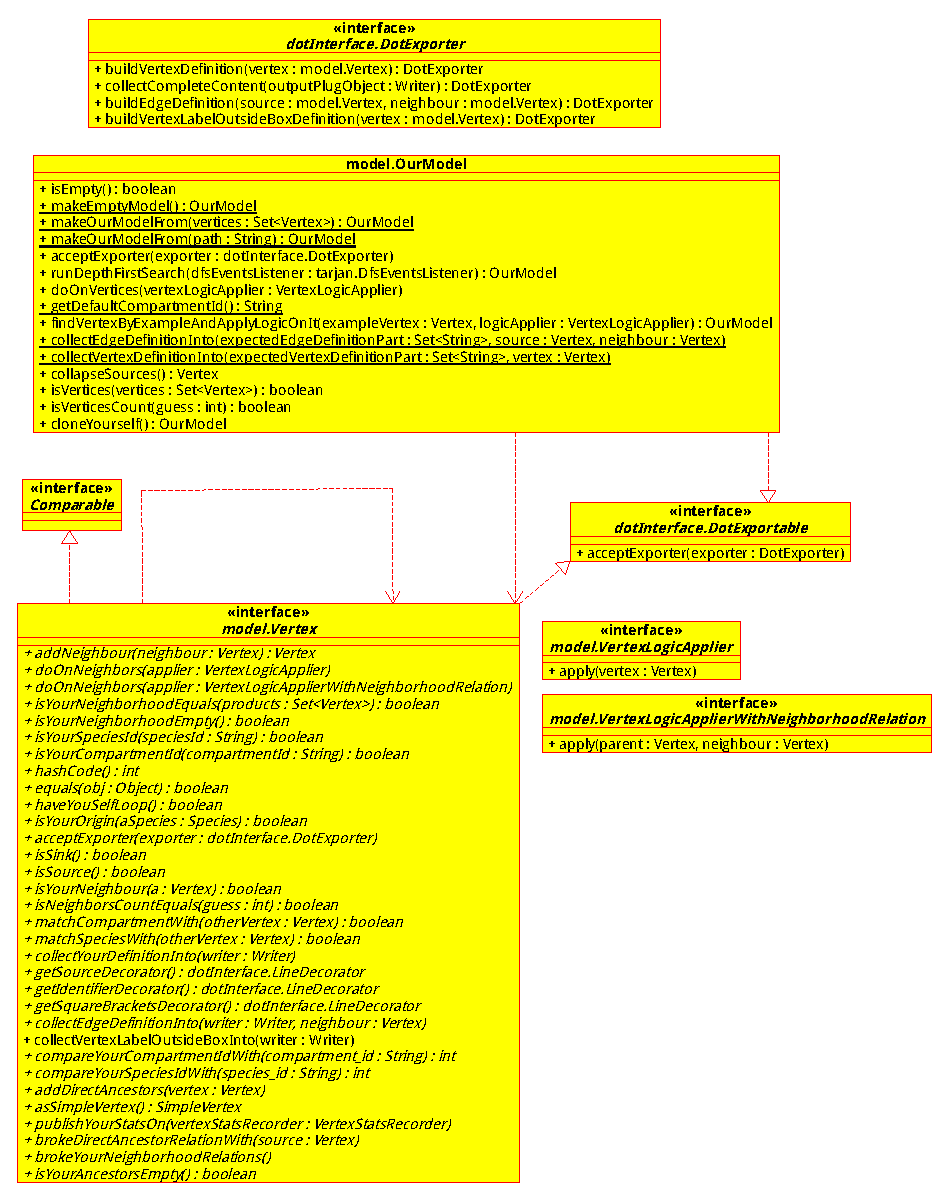
\includegraphics{packages/vertex-interface-class-diagram.eps} 
  \caption{dotInterface package's classes}
  \label{fig:dot-interface-package-classes}
\end{figure}

\begin{paragraph}{DotExporter}
  Il contratto \emph{DotExporter} definisce quali sono i messaggi deve
  essere in grado di comprendere un esportatore per costruire
  documenti in formato dot lavorando su un grafo condificato con le
  astrazioni di \emph{Vertex}.

  I messaggi definiti in \emph{DotExporter} riguardano le componenti
  basilari che si possono rappresentare graficamente di un grafo,
  ovvero il vertice, l'arco ed una eventuale etichetta per il vertice
  (per il nostro lavoro non \`e stato necessario introdurre
  un'etichetta anche per gli archi). Riporto il codice per maggior
  chiarezza:
  \begin{lstlisting}
public interface DotExporter extends DotDocumentPartHandler {
  DotExporter buildVertexDefinition(Vertex vertex);
  DotExporter collectCompleteContent(Writer outputPlugObject);
  DotExporter buildEdgeDefinition(Vertex source, Vertex neighbour);
  DotExporter buildVertexLabelOutsideBoxDefinition(Vertex vertex);
}

public interface DotExportable {
  void acceptExporter(DotExporter exporter);
}

  \end{lstlisting}

  Per non accoppiare in modo forte la modalit\`a di salvataggio
  dell'output nel codice degli implementatori, si espone anche un
  messaggio che porta come argomento un oggetto di tipo \emph{Writer}
  appartenente alla libreria di \emph{io} fornita in \emph{openjdk},
  che \`e possibile utilizzare come destinazione di tutte le
  informazioni che andranno a comporre il documento dot finale. 

  Questo non limita l'insieme di destinazioni dell'output, bensi
  lascia aperte molte strade, ed eventuali client del contratto
  \emph{DotExporter} potranno utilizzare i propri oggetti come
  destinazione dell'output, magari da usare per successive
  computazioni. Nelle nostre implementazioni abbiamo usato quasi
  sempre oggetti di tipo \emph{FileWriter} come destinazioni concrete.
\end{paragraph}

\begin{paragraph}{DotExportable}
  Questo contratto permette di definire quali resposabilit\`a devono
  essere implementate affinch\`e un oggetto sia possibile esportarlo
  in formato dot. 

  Non \`e un interfaccia molto ricca, ma il solo messaggio
  \emph{acceptExporter} \`e sufficiente per catturare la nostra
  idea. Questa struttura si avvicina molto a quella che viene esposta
  per il pattern \emph{Visitor} in \footnote{aggiungere qui
    riferimento alla pagina del visitor in Design Pattern}, anche se
  la nostra implementazione non la ricalca fedelmente: il taglio che
  abbiamo voluto dare alla coppia \emph{DotExporter} e
  \emph{DotExportable} usa sempre come idea di fondo il \emph{double
    dispatch}, con la differenza di non esporre nel contratto
  \emph{DotExporter} metodi relativi alla classi concrete di
  \emph{Vertex}, ma avendo un solo messaggio
  \emph{buildVertexDefinition} (come si vede nel metodo sopra
  riportato).
\end{paragraph}




